\chapter{计算预算与方法选择}
\label{chap:sampling-budget-method-selection}

设要计算$X\sim\operatorname{Exp}(1)$超过$4$的概率$I=\mathbb{P}(X>4)=\mathrm{e}^{-4}\approx0.0183$，要求在$95\%$的把握下相对误差不超过$10\%$，可用的计算量折合$10^{5}$次函数求值。前几章给了很多工具：可以直接平均示性函数，可以改用指数分布$\operatorname{Exp}(\lambda)$作建议分布做重要性采样，也可以先花一些计算量做试运行，再决定$\lambda$。哪一种能在预算内完成任务？“相对误差$10\%$”是不是合适的要求？试运行该花多少？什么时候可以停下来报告结果？

这些问题不是新的数学对象，而是把前四章的结论放到同一本账上。第~\ref{chap:sample-generation}章给出生成样本的各种办法，第~\ref{chap:monte-carlo-integration-error}章说明样本平均的偏差与波动怎样估计，第~\ref{chap:variance-reduction}章讨论怎样在积分不变的前提下减小方差，第~\ref{chap:expectation-gradient-estimation}章把这些方法推广到含参期望的梯度。每一章都在“其他条件不变”的前提下比较方法；实际计算时，误差要求、样本成本、预备开销和停止方式都要同时考虑。

本章按做一次计算的顺序展开。第~\ref{sec:budget-targets}节先确定要控制什么误差，第~\ref{sec:budget-costs}节统一成本的口径，第~\ref{sec:budget-allocation}节把预算分给试运行、正式计算、多条链或多组随机化，第~\ref{sec:budget-selection}节按可计算的信息选择采样、方差控制与梯度估计方法，第~\ref{sec:budget-stopping}节讨论试运行之后怎样固定方案、何时停止。全章反复使用前几章的几个例子：尾概率$\mathrm{e}^{-4}$及其重要性采样，$\mathrm{e}^{u}$在$[0,1]$上的积分$\mathrm{e}-1$及其方差控制，以$\mathcal{N}(0,1)$为不变分布的自回归链，以及双峰混合$0.3\,\mathcal{N}(-2,0.5^{2})+0.7\,\mathcal{N}(2,1)$。

\section{计算目标与精度要求}
\label{sec:budget-targets}

比较方法之前，先要说清楚算什么、算到什么程度算完。待算的量是固定的数：积分$I=\mathbb{E}_{\pi}[f]$，或者含参期望$J(\bm{\theta})$在某一点的梯度$\nabla J(\bm{\theta})\in\mathbb{R}^{d}$。随机的是计算过程，估计$\hat{I}_n$随所用随机数而变。“精度”因此是对$\hat{I}_n-I$这个随机误差的要求，而同一个误差可以用几种不同的方式来约束。不同的约束会要求很不一样的样本数，有的在目标接近零时还会失去意义。

\paragraph{三种误差口径}
最直接的要求是误差的绝对值$\lvert\hat{I}_n-I\rvert$不超过给定的$\varepsilon$。但$\hat{I}_n$是随机的，任何有限样本都可能偶然偏得很远，所以“误差不超过$\varepsilon$”只能以平均或概率的方式表达。第一种是要求\term{均方误差}（mean squared error）不超过$\varepsilon^{2}$。按第~\ref{chap:monte-carlo-integration-error}章的分解，在$\hat{I}_n$二阶矩有限时
\begin{equation}
  \mathbb{E}\bigl[(\hat{I}_n-I)^{2}\bigr]=\bigl(\mathbb{E}[\hat{I}_n]-I\bigr)^{2}+\operatorname{Var}(\hat{I}_n),
  \label{eq:budget-mse}
\end{equation}
右边第一项是偏差的平方，第二项是随机波动。均方误差把两者放在同一个单位下相加，便于在它们之间权衡。

第二种是指定概率下的误差：给定容差$\varepsilon>0$和允许的失败概率$\delta\in(0,1)$，要求
\begin{equation}
  \mathbb{P}\bigl(\lvert\hat{I}_n-I\rvert>\varepsilon\bigr)\le\delta .
  \label{eq:budget-eps-delta}
\end{equation}
它直接回答“这次计算有多大把握落在容差以内”。两种口径之间有一个总成立的桥：对误差平方用Markov不等式，
\[
  \mathbb{P}\bigl(\lvert\hat{I}_n-I\rvert>\varepsilon\bigr)\le\frac{\mathbb{E}\bigl[(\hat{I}_n-I)^{2}\bigr]}{\varepsilon^{2}} .
\]
所以只要均方误差不超过$\delta\varepsilon^{2}$，式~\eqref{eq:budget-eps-delta}就成立。这一步不需要任何分布假设，代价是保守。

对独立同分布、方差为$\sigma^{2}$的无偏样本平均，$\operatorname{Var}(\hat{I}_n)=\sigma^{2}/n$，上面的充分条件给出样本数
\begin{equation}
  n_{\mathrm{Cheb}}=\frac{\sigma^{2}}{\delta\varepsilon^{2}} .
  \label{eq:budget-n-cheb}
\end{equation}
若改用中心极限定理的正态近似，记$z_{1-\delta/2}$为标准正态的$1-\delta/2$分位数，需要的样本数约为
\begin{equation}
  n_{\mathrm{N}}\approx\frac{z_{1-\delta/2}^{2}\,\sigma^{2}}{\varepsilon^{2}} .
  \label{eq:budget-n-normal}
\end{equation}
后者只是渐近近似，覆盖保证不是有限样本下精确的；前者是有限样本下成立的上界。两者的差别完全来自对$\delta$的依赖：Chebyshev界按$1/\delta$增长，正态近似中的$z_{1-\delta/2}^{2}$只按$\ln(1/\delta)$的量级增长。

以$\mathrm{e}^{u}$在$[0,1]$上的积分$I=\mathrm{e}-1$为例，直接平均$\mathrm{e}^{U}$的单样本方差是
\[
  \sigma^{2}=\frac{\mathrm{e}^{2}-1}{2}-(\mathrm{e}-1)^{2}\approx0.2420 .
\]
取$\varepsilon=0.01$、$\delta=0.05$，由式~\eqref{eq:budget-n-cheb}与式~\eqref{eq:budget-n-normal}，
\[
  n_{\mathrm{Cheb}}=\frac{0.2420}{0.05\times10^{-4}}\approx48\,400,\qquad n_{\mathrm{N}}\approx\frac{1.96^{2}\times0.2420}{10^{-4}}\approx9\,300 .
\]
两者相差约$5.2$倍。图~\ref{fig:budget-n-requirement}(a)画出$\delta$变化时这两个样本数：$\delta$越小，Chebyshev界与正态近似的距离越大。选择哪一个，要看报告需要有限样本的保证，还是可以接受渐近近似。

\begin{BookInlineFigure}
  \centering
  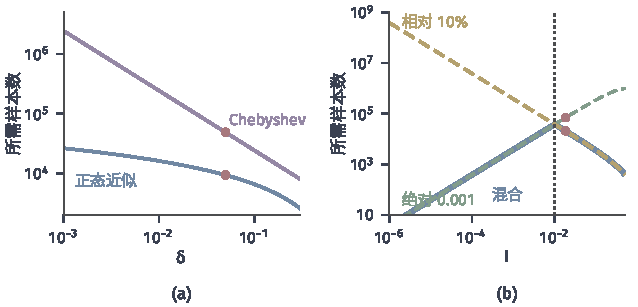
\includegraphics[width=108mm]{figures/07-probability/08-sampling-and-integration/matplotlib/budget-n-requirement/figure.pdf}
  \caption{误差口径决定所需样本数。(a)~积分$\mathrm{e}-1$、容差$\varepsilon=0.01$：紫线为Chebyshev界式~\eqref{eq:budget-n-cheb}，蓝线为正态近似式~\eqref{eq:budget-n-normal}，红点为$\delta=0.05$。(b)~尾概率$I$的直接平均在$95\%$正态近似下所需的样本数：绿色虚线为绝对容差$0.001$，黄色虚线为相对容差$10\%$，蓝色粗线为二者取较宽者的混合容差；竖直点线$I=0.01$是两种容差相等处，红点对应$I=\mathrm{e}^{-4}$。}
  \label{fig:budget-n-requirement}
\end{BookInlineFigure}

梯度的目标是向量$\nabla J(\bm{\theta})\in\mathbb{R}^{d}$，误差用欧氏范数衡量。设估计$\hat{\bm{g}}$的均值为$\bm{m}$，协方差矩阵为$\bm{\Sigma}_{\hat{g}}$，逐分量应用式~\eqref{eq:budget-mse}再相加，得到
\begin{equation}
  \mathbb{E}\bigl[\lVert\hat{\bm{g}}-\nabla J\rVert_2^{2}\bigr]=\lVert\bm{m}-\nabla J\rVert_2^{2}+\operatorname{tr}\bm{\Sigma}_{\hat{g}} .
  \label{eq:budget-vector-mse}
\end{equation}
波动部分是协方差矩阵的迹，即各分量方差之和。若只关心某个方向$\bm{v}$上的变化率，相应的误差只涉及$\bm{v}^{\top}\bm{\Sigma}_{\hat{g}}\bm{v}$，比全向量的要求宽松得多。第~\ref{sec:budget-gradient-choice}节会看到，按迹比较时各种梯度估计的优劣可能与按单个分量比较时不同。

\paragraph{相对误差与接近零的目标}
当待算量很小时，绝对容差$0.001$可能比答案本身还大，于是人们常改用\term{相对误差}（relative error）$\lvert\hat{I}_n-I\rvert/\lvert I\rvert$。对尾概率，相对要求才有意义：$I=\mathrm{e}^{-4}\approx0.0183$时，报告$0.0183\pm0.001$与报告$0.0183\pm0.0002$说明的事情差别不大，但报告$0.0183\pm0.0183$就没有说明任何事。问题出在$I$趋于零时。直接平均示性函数的单样本方差是$I(1-I)$，相对容差$\varepsilon_{\mathrm{rel}}$在正态近似下要求
\[
  n\approx\frac{z^{2}I(1-I)}{(\varepsilon_{\mathrm{rel}}I)^{2}}=\frac{z^{2}(1-I)}{\varepsilon_{\mathrm{rel}}^{2}\,I},
\]
其中$z=1.96$。它随$I\to0$按$1/I$增长；$I=0$时这个要求无法满足，因为任何非零的估计都有无穷大的相对误差。

目标恰为零或可能为零的情形很常见：一个奇函数在对称分布下的期望，参数取到最优点时的梯度，两种方案期望之差在二者一样好时的取值。这时只用相对误差会使计算无限进行下去。实用的写法是给一个\term{混合容差}（mixed tolerance）：
\begin{equation}
  \lvert\hat{I}_n-I\rvert\le\max\bigl\{\varepsilon_{\mathrm{abs}},\ \varepsilon_{\mathrm{rel}}\lvert I\rvert\bigr\} .
  \label{eq:budget-mixed-tolerance}
\end{equation}
目标较大时相对项起作用，目标接近零时绝对项兜底。对梯度，把式中的绝对值换成欧氏范数即可；在参数接近最优点时梯度本身趋于零，这时只有绝对项能给出可以达到的要求。$\varepsilon_{\mathrm{abs}}$不是随意的：它表示“比这更小的差别对使用者已无意义”的尺度，应由任务本身给出。

用尾概率走一遍。$I=\mathrm{e}^{-4}$时单样本方差$I(1-I)\approx0.01798$。绝对容差$0.001$与相对容差$10\%$在正态近似下分别要求
\[
  n_{\mathrm{abs}}\approx\frac{1.96^{2}\times0.01798}{10^{-6}}\approx69\,100,\qquad n_{\mathrm{rel}}\approx\frac{1.96^{2}\times0.9817}{0.01\times0.01832}\approx20\,600 .
\]
混合容差取二者中较宽的$\max\{0.001,0.00183\}=0.00183$，所需样本数就是$20\,600$。图~\ref{fig:budget-n-requirement}(b)把这三条曲线画成$I$的函数：相对容差的曲线在$I\to0$时向上发散，绝对容差的曲线向下，混合容差取二者的较小者，在两种容差相等的$I=0.01$处转折。

还要注意：混合容差里的$\lvert I\rvert$本身未知，实际判断只能用估计值代替。这个代替在估计值远离零时无害，在估计值接近零时会把相对项估得过小或过大，第~\ref{sec:budget-stopping}节讨论依据数据决定何时停止时还会回到这一点。

\paragraph{固定预算与固定精度}
同一个误差要求可以从两个方向提出。一是预算$C$给定，在所有可行方案中使误差最小；二是误差要求给定，使达到它的成本最小。用均方误差写，二者分别是
\begin{equation}
  \min_{\text{方案}}\ \mathrm{MSE}\quad\text{使}\ \text{成本}\le C,
  \qquad
  \min_{\text{方案}}\ \text{成本}\quad\text{使}\ \mathrm{MSE}\le\varepsilon^{2}.
  \label{eq:budget-two-problems}
\end{equation}
对无偏的独立样本平均，两个问题等价。设每个样本的成本为$c$、方差为$\sigma^{2}$，预算$C$可买$n=C/c$个样本，于是
\begin{equation}
  \mathrm{MSE}\cdot C=\frac{\sigma^{2}}{n}\cdot nc=\sigma^{2}c .
  \label{eq:budget-mse-cost-product}
\end{equation}
乘积$\sigma^{2}c$与预算无关：给定预算时误差是$\sigma^{2}c/C$，给定误差时成本是$\sigma^{2}c/\varepsilon^{2}$，哪个方案的$\sigma^{2}c$小，它在两种提法下都更好。第~\ref{sec:budget-costs}节会把$\sigma^{2}c$作为比较的基本量。

有偏差时情况不同。偏差不随样本数减小，它通常由方法的某个参数控制，例如数值离散的步长；而缩小偏差往往使每个有效样本更贵。这时固定预算与固定精度的答案都要在偏差和波动之间折中，而且固定精度的问题可能对某些参数根本无解：若偏差本身已经超过$\varepsilon$，增加样本只会把误差压到偏差为止。

下面用第~\ref{chap:monte-carlo-integration-error}章的近似链说明这种折中。目标是$\pi=\mathcal{N}(0,1)$，被积函数$f(x)=x^{2}$，$I=1$。用步长$h\in(0,1)$的链
\begin{equation}
  X^{(t+1)}=(1-h)X^{(t)}+\sqrt{2h}\,\varepsilon^{(t)},\qquad\varepsilon^{(t)}\sim\mathcal{N}(0,1)\ \text{独立},
  \label{eq:budget-ula-chain}
\end{equation}
每步成本记为$1$。这条链的不变分布不是目标：对平稳的方差$v$，由$v=(1-h)^{2}v+2h$解得$v=2/(2-h)$。于是平稳时的偏差
\[
  b(h)=v-1=\frac{h}{2-h}.
\]

再算波动。记$\rho=1-h$。平稳的高斯自回归链中，$X^{(0)}$与$X^{(k)}$是协方差为$v\rho^{k}$的联合高斯变量，由高斯四阶矩公式，
\[
  \operatorname{Cov}\bigl((X^{(0)})^{2},(X^{(k)})^{2}\bigr)=2\bigl(v\rho^{k}\bigr)^{2}=2v^{2}\rho^{2k}.
\]
代入第~\ref{chap:monte-carlo-integration-error}章的长期方差（$\gamma_{0}$加上各阶自协方差之和的两倍），对几何级数求和，得到
\[
  \sigma_{\mathrm{LR}}^{2}(h)=2v^{2}\Bigl(1+2\sum_{k\ge1}\rho^{2k}\Bigr)=\frac{2v^{2}(1+\rho^{2})}{1-\rho^{2}}=\frac{2v^{2}\bigl(1+(1-h)^{2}\bigr)}{h(2-h)} .
\]
从平稳状态启动、运行$B$步时，均方误差在$B$较大时为
\begin{equation}
  \mathrm{MSE}(h,B)\approx b(h)^{2}+\frac{\sigma_{\mathrm{LR}}^{2}(h)}{B} .
  \label{eq:budget-ula-mse}
\end{equation}
步长越小，偏差越小，但链的相关越强，波动越大。

对小$h$取主项，$b(h)\approx h/2$，$\sigma_{\mathrm{LR}}^{2}(h)\approx2/h$，于是
\[
  \mathrm{MSE}(h,B)\approx\frac{h^{2}}{4}+\frac{2}{hB}.
\]
对$h$求导并令其为零，$h/2-2/(h^{2}B)=0$，解得最优步长和最小均方误差
\begin{equation}
  h^{\ast}\approx\Bigl(\frac{4}{B}\Bigr)^{1/3},\qquad\mathrm{MSE}^{\ast}\approx\frac34\cdot4^{2/3}B^{-2/3}\approx1.89\,B^{-2/3}.
  \label{eq:budget-ula-opt}
\end{equation}
均方根误差按$B^{-1/3}$下降，比无偏样本平均的$B^{-1/2}$慢。原因是每增加预算，最优安排都要把一部分花在缩小步长上，而不是全部用于平均。

图~\ref{fig:budget-ula-tradeoff}(a)按式~\eqref{eq:budget-ula-mse}的精确表达式画出三种预算下的均方误差：左侧是波动主导，右侧贴近偏差平方$b(h)^{2}$，红点是最优步长。$B=10^{4}$时数值最优$h^{\ast}\approx0.071$，均方误差约$0.0043$，均方根误差约$0.065$；从$\mathcal{N}(0,1)$直接独立抽样时$\operatorname{Var}(X^{2})=2$，同样预算的均方根误差是$\sqrt{2/10^{4}}\approx0.014$。图~\ref{fig:budget-ula-tradeoff}(b)比较两种方法达到均方根误差$\varepsilon=0.01$所需的预算：精确采样需要$2/\varepsilon^{2}=2\times10^{4}$步，近似链即使每次都取最优步长也需要约$2.6\times10^{6}$步。

\begin{BookInlineFigure}
  \centering
  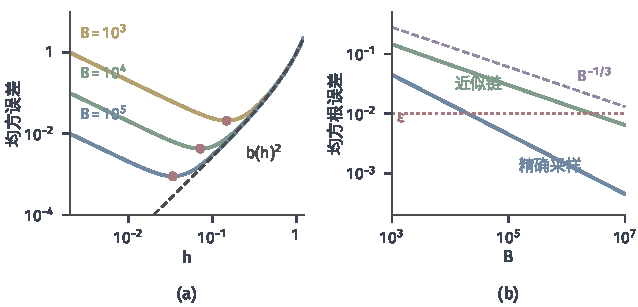
\includegraphics[width=108mm]{figures/07-probability/08-sampling-and-integration/matplotlib/budget-ula-tradeoff/figure.pdf}
  \caption{近似链~\eqref{eq:budget-ula-chain}在偏差与波动之间的折中，$f(x)=x^{2}$，目标$\mathcal{N}(0,1)$，从平稳状态启动。(a)~三种预算$B$下的均方误差随步长$h$变化，深灰虚线为偏差平方$b(h)^{2}$，红点为最优步长。(b)~均方根误差随预算变化：蓝线为独立精确抽样，绿线为每个预算下取最优步长的近似链，紫色虚线为$B^{-1/3}$参考斜率，红色点线为容差$\varepsilon=0.01$。}
  \label{fig:budget-ula-tradeoff}
\end{BookInlineFigure}

这个例子还说明，式~\eqref{eq:budget-two-problems}两种提法的结论都依赖偏差项是否存在。对无偏方法，只需比较$\sigma^{2}c$；对有偏方法，必须同时选择控制偏差的参数，固定精度的要求会把预算推到偏差允许的范围。式~\eqref{eq:budget-ula-mse}忽略了初值的影响，从非平稳状态启动时还要加上第~\ref{chap:monte-carlo-integration-error}章所说的初始偏差，它在这里按$1/(hB)$衰减，不改变$B^{-1/3}$的量级。

\section{计算成本}
\label{sec:budget-costs}

式~\eqref{eq:budget-mse-cost-product}说明，无偏方法之间比较的是“单样本方差乘单样本成本”。可是“一个样本”在不同方法里含义不同：拒绝采样的一个输出要先生成并淘汰若干候选，Markov链每步都产生一个状态但相邻状态高度相关，有的方法在抽第一个样本之前就要做一次矩阵分解或一轮试运行。要让比较公平，就要把这些开销记在同一本账上，并且明确“成本”是按什么单位计的。

\paragraph{成本的组成}
一次随机计算的开销可以分成三类。第一类是每次迭代的操作：生成基础随机数，按建议分布生成候选，计算目标密度、密度比或梯度，计算被积函数。第二类把迭代换算成输出：拒绝采样平均要做若干次迭代才输出一个样本，抽稀的链每$k$步才保存一个状态。第三类只发生一次或每条链一次：矩阵分解、试运行与建议分布的拟合、控制系数或分层方案的预估，以及链开始时为摆脱初值而舍弃的$b$步。

记一次迭代的成本为$c_{\mathrm{it}}$，一个输出样本的成本为$c_{\mathrm{out}}$，一次性开销为$C_{0}$。输出$n$个样本的总成本是
\begin{equation}
  C=C_{0}+b\,c_{\mathrm{it}}+n\,c_{\mathrm{out}} .
  \label{eq:budget-total-cost}
\end{equation}
图~\ref{fig:budget-cost-ledger}把这几项的关系画成一张账：单项操作合成一次迭代，迭代乘以候选数或抽稀间隔得到输出样本，输出样本再乘以相关性的影响得到下文的有效样本。计成本的单位可以是运行时间，也可以是某种主导操作的次数（如目标密度的计算次数）。用操作次数便于复现和推导，用时间更贴近实际，二者在向量化、缓存或并行时可能给出不同的排序，比较前要说明用的是哪一种。

\begin{BookInlineFigure}
  \centering
  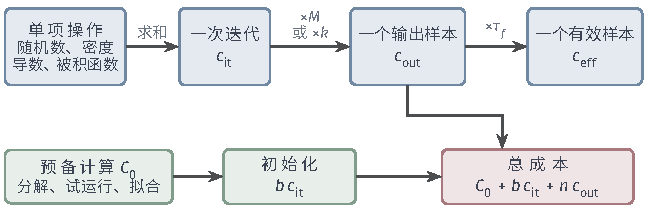
\includegraphics[width=110mm]{figures/07-probability/08-sampling-and-integration/tikz/budget-cost-ledger/figure.pdf}
  \caption{一次随机计算的成本账。上排是按单位累积的成本：单项操作合成一次迭代$c_{\mathrm{it}}$，拒绝采样乘以平均候选数$M$、抽稀乘以间隔$k$得到一个输出样本$c_{\mathrm{out}}$，相关链再乘以$\tau_{f}$得到针对被积函数$f$的一个有效样本。下排是只计一次的开销：预备计算$C_{0}$和每条链初始化舍弃的$b$步，它们与$n$个输出的成本合成总成本~\eqref{eq:budget-total-cost}。}
  \label{fig:budget-cost-ledger}
\end{BookInlineFigure}

\paragraph{工作量归一化方差}
设某个无偏方法的输出相互独立，单样本方差为$\sigma^{2}$，单样本成本为$c$，一次性开销为$C_{0}$，暂不考虑初始化。总预算$C>C_{0}$可买$n=(C-C_{0})/c$个样本（忽略取整），估计的方差为
\begin{equation}
  \operatorname{Var}(\hat{I})=\frac{\sigma^{2}c}{C-C_{0}} .
  \label{eq:budget-var-budget}
\end{equation}
称$\sigma^{2}c$为\term{工作量归一化方差}（work-normalized variance）。预算远大于$C_{0}$时，它是比较两种方法的唯一量：方法甲优于方法乙，当且仅当$\sigma_{\text{甲}}^{2}c_{\text{甲}}<\sigma_{\text{乙}}^{2}c_{\text{乙}}$。单看方差或单看成本都会误判：方差小一半而每个样本贵三倍的方法，在同样预算下反而更差。

一次性开销使比较依赖预算。设方法乙没有预备开销，方法甲有$C_{0}>0$且$\sigma_{\text{甲}}^{2}c_{\text{甲}}<\sigma_{\text{乙}}^{2}c_{\text{乙}}$。由式~\eqref{eq:budget-var-budget}，甲的方差较小当且仅当
\[
  \frac{\sigma_{\text{甲}}^{2}c_{\text{甲}}}{C-C_{0}}<\frac{\sigma_{\text{乙}}^{2}c_{\text{乙}}}{C},
\]
整理得
\begin{equation}
  C>C_{\times}=\frac{C_{0}\,\sigma_{\text{乙}}^{2}c_{\text{乙}}}{\sigma_{\text{乙}}^{2}c_{\text{乙}}-\sigma_{\text{甲}}^{2}c_{\text{甲}}} .
  \label{eq:budget-crossover}
\end{equation}
预算低于$C_{\times}$时，花在准备上的成本收不回来。

以第~\ref{chap:variance-reduction}章的尾概率为例。直接平均的$\sigma^{2}=I(1-I)\approx0.01798$，每个样本成本记为$1$；从$\operatorname{Exp}(1/4)$抽样的重要性采样单样本方差约$0.001749$，每个样本成本记为$1.5$，选定建议分布的预备开销记为$C_{0}=2000$。两者的工作量归一化方差分别为
\[
  0.01798\times1=0.01798,\qquad0.001749\times1.5\approx0.002623,
\]
大预算下重要性采样约好$6.9$倍。代入式~\eqref{eq:budget-crossover}，
\[
  C_{\times}=\frac{2000\times0.01798}{0.01798-0.002623}\approx2342 .
\]
本章开头的预算$10^{5}$远超过它，准备是值得的。

\paragraph{拒绝候选与矩阵分解}
拒绝采样的每个候选被接受的概率是$1/M$，$M$为包络常数（第~\ref{chap:sample-generation}章）。各候选独立，所以得到一个输出所需的候选数$N$服从参数$1/M$的几何分布，$\mathbb{P}(N=j)=(1-1/M)^{j-1}/M$，其均值为
\[
  \mathbb{E}[N]=\sum_{j\ge1}j\Bigl(1-\frac1M\Bigr)^{j-1}\frac1M=\frac{1/M}{(1/M)^{2}}=M .
\]
若每个候选要生成一次建议样本（成本$c_{q}$）、计算一次接受判据（成本$c_{\mathrm{acc}}$），被接受的样本还要计算一次被积函数（成本$c_{f}$），则
\begin{equation}
  c_{\mathrm{out}}=M\,(c_{q}+c_{\mathrm{acc}})+c_{f} .
  \label{eq:budget-rejection-cost}
\end{equation}
被淘汰的候选不产生输出，但其成本全额计入。$M$随维数增长时，这一项可能成为全部成本的主体。

生成$\mathcal{N}(\bm{\mu},\bm{\Sigma})$的样本时，要先把$d\times d$的协方差矩阵分解为$\bm{\Sigma}=\bm{L}\bm{L}^{\top}$，此后每个样本是$\bm{\mu}+\bm{L}\bm{Z}$。按\BookChapterRef{chap:direct-linear-solvers}{卷二第12章“线性方程的直接求解”}，Cholesky分解约需$d^{3}/3$次乘加，下三角矩阵乘向量约需$d^{2}$次。抽$n$个样本时，平均到每个样本的乘加次数约为
\[
  \frac{d^{3}/3}{n}+d^{2}=d^{2}\Bigl(1+\frac{d}{3n}\Bigr).
\]
$n$远大于$d$时分解的开销可以忽略；$n$与$d$相当或更小时（例如$d=1000$只抽$100$个样本），分解占了大部分成本，这时比较方法必须把$C_{0}$计入，而不能只看每个样本的$d^{2}$。

\paragraph{迭代、输出样本与有效样本}
Markov链每步输出一个状态，相邻状态相关，保存下来的状态数不能直接当作样本数。设链平稳，被积函数$f$的单步方差为$\gamma_{0}$，长期方差为$\sigma_{\mathrm{LR}}^{2}$，记
\begin{equation}
  \tau_{f}=\frac{\sigma_{\mathrm{LR}}^{2}}{\gamma_{0}},\qquad N_{\mathrm{eff}}=\frac{N}{\tau_{f}} .
  \label{eq:budget-tau}
\end{equation}
这里的$N_{\mathrm{eff}}$就是第~\ref{chap:monte-carlo-integration-error}章的有效样本量：$N$步相关平均的渐近方差$\sigma_{\mathrm{LR}}^{2}/N$等于$N_{\mathrm{eff}}$个独立样本的方差$\gamma_{0}/N_{\mathrm{eff}}$。于是忽略初始化时，针对$f$的一个有效样本的成本是
\begin{equation}
  c_{\mathrm{eff}}=c_{\mathrm{it}}\,\tau_{f},
  \label{eq:budget-eff-cost}
\end{equation}
相关链的工作量归一化方差是
\[
  \gamma_{0}\,c_{\mathrm{eff}}=\gamma_{0}c_{\mathrm{it}}\tau_{f}=\sigma_{\mathrm{LR}}^{2}c_{\mathrm{it}} .
\]

$\tau_{f}$属于“链与被积函数”这一对，而不是只属于链。以平稳自回归链
\begin{equation}
  X^{(t+1)}=\rho X^{(t)}+\sqrt{1-\rho^{2}}\,\varepsilon^{(t)},\qquad\varepsilon^{(t)}\sim\mathcal{N}(0,1)\ \text{独立}
  \label{eq:budget-ar1}
\end{equation}
为例，目标$\mathcal{N}(0,1)$。对$f(x)=x$，$\gamma_{k}=\rho^{k}$；对$f(x)=x^{2}$，$\gamma_{k}=2\rho^{2k}$。分别对几何级数求和，得到
\[
  \tau_{x}=\frac{1+\rho}{1-\rho},\qquad\tau_{x^{2}}=\frac{1+\rho^{2}}{1-\rho^{2}} .
\]
$\rho=0.9$时$\tau_{x}=19$，$\tau_{x^{2}}\approx9.53$：同一条链的同一段记录，估计$\mathbb{E}[X^{2}]$时的有效样本数约是估计$\mathbb{E}[X]$时的两倍。图~\ref{fig:budget-ess-thinning}(a)画出每步的有效样本数$1/\tau_{f}$随$\rho$的变化。

\begin{BookInlineFigure}
  \centering
  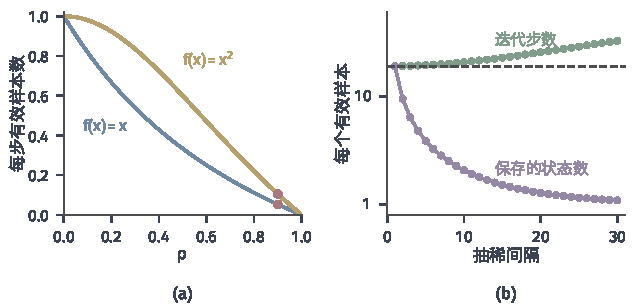
\includegraphics[width=108mm]{figures/07-probability/08-sampling-and-integration/matplotlib/budget-ess-thinning/figure.pdf}
  \caption{平稳自回归链（目标$\mathcal{N}(0,1)$）的有效样本。(a)~每步迭代提供的有效样本数$1/\tau_{f}$：蓝线$f(x)=x$，黄线$f(x)=x^{2}$，红点为$\rho=0.9$。(b)~$\rho=0.9$、$f(x)=x$时每隔$k$步保存一个状态：绿线为每个有效样本所需的迭代步数，紫线为所需保存的状态数，深灰虚线为不抽稀时的$19$步。}
  \label{fig:budget-ess-thinning}
\end{BookInlineFigure}

保存时常做\term{抽稀}（thinning）：每$k$步只保存一个状态。抽稀后的序列仍是自回归链，系数为$\rho^{k}$，长度为$N/k$。对$f(x)=x$，每个有效样本需要保存$(1+\rho^{k})/(1-\rho^{k})$个状态，相应的迭代步数是
\[
  k\,\frac{1+\rho^{k}}{1-\rho^{k}} .
\]
$\rho=0.9$、$k=10$时，前者约$2.07$，后者约$20.7$，比不抽稀的$19$步还多。图~\ref{fig:budget-ess-thinning}(b)显示了这一点：抽稀减少存储，不减少计算，对这个例子还略微损失精度。只有被积函数本身很贵，例如每次求值的成本$c_{f}$远大于一步转移的成本时，抽稀才能节省计算，因为这时每个保存状态的成本是$k\,c_{\mathrm{it}}+c_{f}$，适当的$k$可以减少昂贵的求值次数。

链的初始化另有成本。每条链舍弃前$b$步，花费$b\,c_{\mathrm{it}}$，这一项不随保存的样本数摊薄，启动的链越多，总的初始化成本越高。第~\ref{sec:budget-allocation}节比较多次启动与单链延长时会用到这一点。

\paragraph{三种采样方式的成本比较}
把上面的账用到第~\ref{chap:sample-generation}章的双峰混合
\[
  \pi=0.3\,\mathcal{N}(-2,0.5^{2})+0.7\,\mathcal{N}(2,1)
\]
上，被积函数取$f(x)=x$。这时
\[
  I=0.3\times(-2)+0.7\times2=0.8,\qquad\operatorname{Var}_{\pi}(f)=0.3\times4.25+0.7\times5-0.8^{2}=4.135 .
\]

作为教学约定，取成本单位：一个均匀数记$1$，一个标准高斯数记$2$，计算一次混合密度记$4$（两个指数），计算一次单个高斯包络的密度记$2$，计算一次$f$记$1$。三种方式的单样本成本如下。
\begin{itemize}
  \item 分步生成：先用一个均匀数选成分，再生成一个高斯数，最后算$f$，$c_{\mathrm{out}}=1+2+1=4$，样本独立，$\tau_{f}=1$。
  \item 拒绝采样：在网格上选使$M$最小的高斯包络，得到$\mathcal{N}(0.25,2.2^{2})$，$M\approx2.29$，接受率约$0.44$。每个候选要一个高斯数、一次包络密度、一次目标密度和一个均匀数，共$9$，由式~\eqref{eq:budget-rejection-cost}，$c_{\mathrm{out}}\approx9\times2.29+1\approx21.7$。
  \item 随机游走Metropolis：每步一个高斯数、一次目标密度、一个均匀数和一次$f$，$c_{\mathrm{it}}=8$。$\tau_{f}$由$10^{6}$步链的分块均值估计，步长$s=1,2.5,4$时分别约为$66$、$8.5$、$6.5$。
\end{itemize}

由式~\eqref{eq:budget-eff-cost}，Metropolis每个有效样本的成本分别约为$527$、$68$、$52$。图~\ref{fig:budget-sampler-costs}(b)把五个数放在对数坐标上：对这个一维目标，分步生成比最好的链便宜十几倍，拒绝采样介于其间。若只按“保存的状态数”比较，Metropolis每步成本$8$只是拒绝采样的约三分之一，结论正好相反。图~\ref{fig:budget-sampler-costs}(a)给出原因：步长$s=1$时，状态要在两个峰之间往返，自相关衰减很慢；步长较大时接受率降低，但跨峰更容易，$\tau_{f}$反而小得多。

\begin{BookInlineFigure}
  \centering
  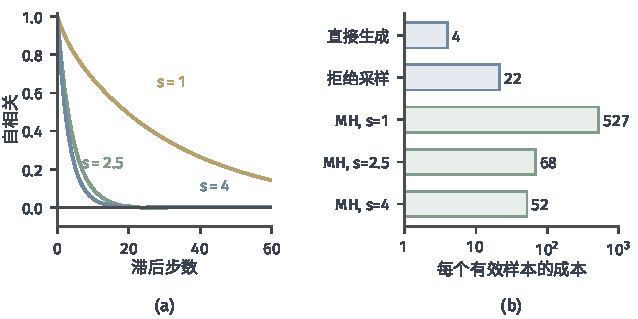
\includegraphics[width=108mm]{figures/07-probability/08-sampling-and-integration/matplotlib/budget-sampler-costs/figure.pdf}
  \caption{双峰混合$0.3\,\mathcal{N}(-2,0.5^{2})+0.7\,\mathcal{N}(2,1)$、$f(x)=x$时三种采样方式的成本（教学约定的操作计数）。(a)~随机游走Metropolis的自相关函数，三条线对应步长$s=1,2.5,4$，各由$10^{6}$步链计算。(b)~每个有效样本的成本：蓝色为独立样本，绿色为Metropolis（每步成本乘以估计的$\tau_{f}$）。}
  \label{fig:budget-sampler-costs}
\end{BookInlineFigure}

这里的$\tau_{f}$是从一段有限记录估计的，它本身有误差，而且只有在链确实走遍两个峰时才可信；第~\ref{sec:budget-stopping}节会看到有限记录可能完全没有发现某个峰。比较结论还依赖成本单位：若目标密度极贵而高斯数几乎免费，各项的比例会改变。账本的作用是让这些假设明确可查，而不是给出与假设无关的排名。

\section{预算分配}
\label{sec:budget-allocation}

有了成本账，下一个问题是同一笔预算怎样分。几乎每种改进都要求先花一部分计算去“了解问题”：重要性采样要先拟合建议分布，控制变量要先估计系数，分层要先知道各层的波动，Markov链要先跑掉初值的影响。花得太少，方案选得差；花得太多，留给正式计算的就少了。成组随机化还有另一种分法：总点数一定时，每组放多少点、重复多少组。

\paragraph{试运行与正式计算}
设总预算为$C$。先用$n_{0}$个试运行样本（每个成本$c_{0}$）确定方法的参数$\hat{\lambda}$，再用剩下的预算按$\hat{\lambda}$做正式计算，每个正式样本成本为$c$。正式计算使用与试运行独立的新随机数，所以在给定试运行结果的条件下，正式估计仍是无偏的独立样本平均（第~\ref{chap:variance-reduction}章对固定建议后的估计证明了这一点），其条件方差为$v(\hat{\lambda})c/(C-n_{0}c_{0})$，这里$v(\lambda)$是参数取$\lambda$时的单样本方差。对试运行取期望，最终估计的方差是
\begin{equation}
  \operatorname{Var}(\hat{I})=\frac{\mathbb{E}\bigl[v(\hat{\lambda})\bigr]\,c}{C-n_{0}c_{0}} .
  \label{eq:budget-pilot-var}
\end{equation}
分子随$n_{0}$增大而减小，因为参数估得更准；分母也随$n_{0}$增大而减小，因为正式计算的预算变少。

为看清两种作用怎样平衡，设$\hat{\lambda}$随$n_{0}\to\infty$收敛到$\bar{\lambda}$，$v$在$\bar{\lambda}$附近光滑，且$\hat{\lambda}-\bar{\lambda}$的均方按$1/n_{0}$缩小。

若$\bar{\lambda}$是$v$的最小点，展开到二阶，一阶项消失；若不是，$\hat{\lambda}$的偏差与波动也只在$1/n_{0}$阶贡献额外方差。两种情形都可以写成
\[
  \mathbb{E}\bigl[v(\hat{\lambda})\bigr]\approx\bar{v}+\frac{a}{n_{0}},
\]
其中$\bar{v}=v(\bar{\lambda})$，$a>0$概括参数估计误差的影响。代入式~\eqref{eq:budget-pilot-var}，要最小化
\[
  g(n_{0})=\frac{\bar{v}+a/n_{0}}{C-n_{0}c_{0}} .
\]
令$g'(n_{0})=0$，即
\[
  -\frac{a}{n_{0}^{2}}\,(C-n_{0}c_{0})+c_{0}\Bigl(\bar{v}+\frac{a}{n_{0}}\Bigr)=0,
\]
两边乘以$n_{0}^{2}$并整理，得到
\[
  c_{0}\bar{v}\,n_{0}^{2}+2ac_{0}\,n_{0}-aC=0 .
\]
取正根，并在$C$远大于$ac_{0}/\bar{v}$时保留主项，得到
\begin{equation}
  n_{0}^{\ast}\approx\sqrt{\frac{aC}{c_{0}\bar{v}}},\qquad\frac{n_{0}^{\ast}c_{0}}{C}\approx\sqrt{\frac{ac_{0}}{\bar{v}C}} .
  \label{eq:budget-pilot-opt}
\end{equation}
试运行的样本数按$\sqrt{C}$增长，占总预算的比例按$1/\sqrt{C}$缩小。预算越大，越值得把参数估准，但越不必为此花上一个固定的比例。

用本章开头的尾概率演示。试运行从覆盖尾部的$q_{0}=\operatorname{Exp}(1/2)$抽样，每个样本对积分的贡献为$c_{i}=\mathbf{1}_{\{Y_i>4\}}p(Y_i)/q_{0}(Y_i)$。第~\ref{chap:variance-reduction}章说明理想的建议分布正比于$\mathbf{1}_{\{x>4\}}\mathrm{e}^{-x}$，其均值为$5$。在指数族$\operatorname{Exp}(\lambda)$中，用贡献加权的均值去匹配$1/\lambda$：
\[
  \hat{\lambda}=\frac{\sum_{i}c_i}{\sum_{i}c_iY_i},
\]
试运行没有样本超过$4$时保留$\lambda=1/2$。$n_{0}\to\infty$时$\hat{\lambda}\to1/5$，此时单样本方差$v(0.2)\approx0.001738$，与族内最优$\lambda^{\ast}\approx0.219$处的$v^{\ast}\approx0.001730$只差$0.5\%$。试运行与正式样本的成本都记为$1.5$。

图~\ref{fig:budget-pilot-size}画出三种预算下最终的相对均方根误差$\sqrt{\operatorname{Var}(\hat{I})}/I$随$n_{0}$的变化，条件方差用精确公式计算，对试运行的期望用模拟（种子$7$）。三条曲线的谷底都很平：$C=1500$时最好的$n_{0}$约为$37$，相对均方根误差约$0.074$，比已知最优建议分布的$0.072$只差一点；$n_{0}$小到$5$时误差约$0.084$，只高出约$14\%$；$n_{0}$大到预算的$70\%$时误差约$0.131$，高出约$78\%$。作为对照，同样预算的直接平均相对误差约为$0.19$。三种预算的最优$n_{0}$随$C$右移，但远慢于$C$本身的增长，与式~\eqref{eq:budget-pilot-opt}一致。

\begin{BookInlineFigure}
  \centering
  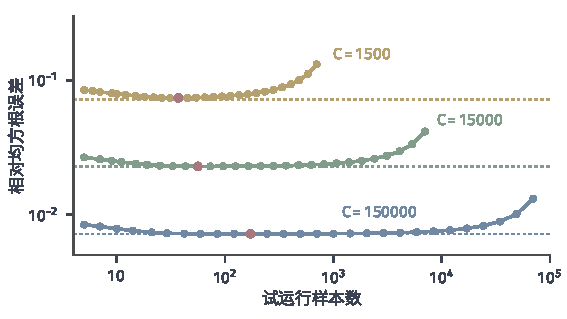
\includegraphics[width=96mm]{figures/07-probability/08-sampling-and-integration/matplotlib/budget-pilot-size/figure.pdf}
  \caption{试运行规模与最终精度。目标$I=\mathbb{P}(X>4)$，$X\sim\operatorname{Exp}(1)$；试运行从$\operatorname{Exp}(1/2)$抽取$n_{0}$个样本拟合$\lambda$，正式计算用新随机数从$\operatorname{Exp}(\hat{\lambda})$抽样，每个样本成本$1.5$。三条曲线对应总预算$C=1500$、$15000$、$150000$，点线为已知最优$\lambda^{\ast}$时的误差，红点为各曲线的最小点。}
  \label{fig:budget-pilot-size}
\end{BookInlineFigure}

这个例子的拟合问题很容易，只有一个参数，所以谷底特别平。参数多、贡献区域分散时，$a$会大得多，过小的试运行可能根本没有观察到某个贡献区域，这时式~\eqref{eq:budget-pilot-opt}所依据的“误差按$1/n_{0}$缩小”还没有开始成立。第~\ref{sec:budget-stopping}节讨论这种情形。

\paragraph{预备开销的分摊}
控制变量的系数也可以由试运行估计。用$n_{0}$个独立的试运行样本估计$\hat{\beta}$，再用新样本计算$f-\hat{\beta}(h-\mathbb{E}h)$的平均，给定$\hat{\beta}$时正式估计无偏，方差为$\operatorname{Var}\bigl(f-\hat{\beta}h\bigr)/n$，分析与式~\eqref{eq:budget-pilot-var}相同。若用同一批样本既估系数又求平均，省下了试运行，却引入$1/n$阶的有限样本偏差（第~\ref{chap:variance-reduction}章），预算较大时这一偏差相对于波动可以忽略，预算很小时则要计入。

分层采样把预备开销与分配规则联系在一起。设$K$层的概率为$p_k$，层内单样本方差为$\sigma_k^{2}$，层内每个样本的成本为$c_k$，第$k$层抽$n_k$个样本。

分层估计的方差与总成本分别是
\[
  \sum_{k=1}^{K}\frac{p_k^{2}\sigma_k^{2}}{n_k},\qquad\sum_{k=1}^{K}n_kc_k=C .
\]
由Cauchy--Schwarz不等式，
\[
  \Bigl(\sum_{k}p_k\sigma_k\sqrt{c_k}\Bigr)^{2}=\Bigl(\sum_{k}\frac{p_k\sigma_k}{\sqrt{n_k}}\cdot\sqrt{n_kc_k}\Bigr)^{2}\le\sum_{k}\frac{p_k^{2}\sigma_k^{2}}{n_k}\cdot\sum_{k}n_kc_k,
\]
等号当且仅当$\sqrt{n_kc_k}$与$p_k\sigma_k/\sqrt{n_k}$成比例。于是固定预算下的最优分配与最小方差为
\begin{equation}
  n_k\propto\frac{p_k\sigma_k}{\sqrt{c_k}},\qquad\operatorname{Var}_{\min}=\frac{1}{C}\Bigl(\sum_{k=1}^{K}p_k\sigma_k\sqrt{c_k}\Bigr)^{2} .
  \label{eq:budget-neyman-cost}
\end{equation}

式~\eqref{eq:budget-neyman-cost}要求知道各层的$\sigma_k$和$c_k$，实际只能由试运行估计，而估计的成本与估计误差都要计入。按$n_k\propto p_k$的比例分配不需要这些信息，在样本总数相同时其方差不超过直接平均；把预算从比例分配转向式~\eqref{eq:budget-neyman-cost}，只有在试运行能可靠区分各层波动时才值得。

以$\mathrm{e}^{U}$的$4$层等概率分层为例，各层成本相同，层内标准差依次约为$0.082$、$0.105$、$0.135$、$0.173$。比例分配与式~\eqref{eq:budget-neyman-cost}的最优分配按每个样本折算的方差分别为
\[
  \sum_{k}p_k\sigma_k^{2}\approx0.01653,\qquad\Bigl(\sum_{k}p_k\sigma_k\Bigr)^{2}\approx0.01536,
\]
最优分配把样本按约$0.17:0.21:0.27:0.35$分给四层，只多省约$7\%$。若为估计$\sigma_k$专门做一轮试运行，这点收益很容易被试运行的成本和$\sigma_k$的估计误差抵消；直接平均的$0.2420$到比例分层的$0.0165$才是主要的改进。

\paragraph{多次启动与单链延长}
Markov链的预算$B$（总迭代步数）可以给一条长链，也可以分给$m$条短链，每条$B/m$步，各自舍弃前$b$步。用式~\eqref{eq:budget-ar1}中$\rho=0.9$的自回归链计算，目标$\mathcal{N}(0,1)$，$f(x)=x$，$I=0$，所有链都从$x_{0}=10$启动。这条链的矩可以精确写出：
\[
  \mathbb{E}\bigl[X^{(t)}\bigr]=0.9^{t}x_{0},\qquad\operatorname{Cov}\bigl(X^{(s)},X^{(t)}\bigr)=0.9^{\lvert t-s\rvert}\bigl(1-0.81^{\min(s,t)}\bigr),
\]
于是每种分法的均方误差都可以精确计算。

图~\ref{fig:budget-chain-count}给出$B=2000$时的结果。不舍弃初值（$b=0$）时，一条链的均方误差约$0.0115$，其中偏差约$0.045$；分成$10$条链后偏差升到约$0.45$，均方误差约$0.21$。原因是每条链都带着同样的初值偏差，平均多条链不能抵消它，而每条链越短，初值那一段所占的比例越大。舍弃$b=30$步后，一条链的均方误差约$0.0096$，接近平稳时的$\sigma_{\mathrm{LR}}^{2}/B=19/2000=0.0095$；链数增多，$mb$步的初始化成本吃掉越来越多的预算，$m=50$时均方误差升到约$0.076$。对单峰、链混合良好的目标，只看均方误差，一条长链最省。

单链时舍弃多少步也可以由均方误差估算。设舍弃$b$步后保留$L=B-b$步，初值偏差在平均中留下的部分约为
\[
  \frac{x_{0}}{L}\sum_{t=b+1}^{B}\rho^{t}\approx\frac{x_{0}\rho^{b+1}}{(1-\rho)L},
\]
波动约为$\sigma_{\mathrm{LR}}^{2}/L$。$b$每增加$1$，偏差平方约乘以$\rho^{2}$，减少量约为偏差平方的$2\ln(1/\rho)$倍；波动则因$L$减少$1$而约增加$\sigma_{\mathrm{LR}}^{2}/L^{2}$。在最优的$b$处二者相等，
\[
  2\ln\frac1\rho\cdot\frac{x_{0}^{2}\rho^{2b+2}}{(1-\rho)^{2}L^{2}}=\frac{\sigma_{\mathrm{LR}}^{2}}{L^{2}},
  \qquad\text{即}\qquad
  \rho^{2b+2}=\frac{\sigma_{\mathrm{LR}}^{2}(1-\rho)^{2}}{2x_{0}^{2}\ln(1/\rho)} .
\]
代入$\rho=0.9$、$x_{0}=10$、$\sigma_{\mathrm{LR}}^{2}=19$，右边约为$0.0090$，解得$b\approx21$，与精确计算的最优值$21$一致。舍弃步数只按$\ln x_{0}$增长：初值离目标越远，舍弃越多，但远小于总预算。这个估算要求知道链向目标靠拢的速度$\rho$，一般的链只能由试运行或理论估计。

\begin{BookInlineFigure}
  \centering
  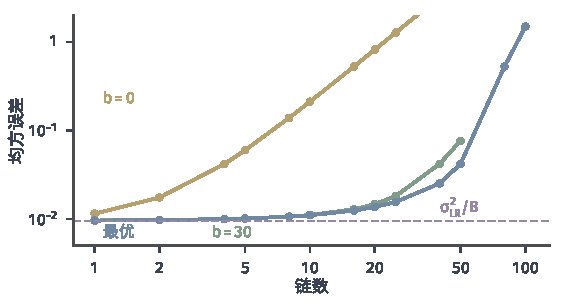
\includegraphics[width=96mm]{figures/07-probability/08-sampling-and-integration/matplotlib/budget-chain-count/figure.pdf}
  \caption{总预算$B=2000$步分给$m$条链时的精确均方误差。自回归链系数$0.9$，目标$\mathcal{N}(0,1)$，$f(x)=x$，每条链从$x_{0}=10$启动并舍弃前$b$步。黄线$b=0$，绿线$b=30$，蓝线对每个$m$取最优$b$；紫色虚线为平稳单链的$\sigma_{\mathrm{LR}}^{2}/B$。}
  \label{fig:budget-chain-count}
\end{BookInlineFigure}

多次启动的价值在别处：它是发现链没有走遍目标的少数手段之一。图~\ref{fig:budget-multistart}在双峰混合$0.3\,\mathcal{N}(-2,0.5^{2})+0.7\,\mathcal{N}(2,1)$上用步长$s=0.5$的随机游走Metropolis，从$-4,-1,1,4$四个分散的初值各跑$500$步。从$-4$与$-1$出发的两条链始终留在左峰，平均约$-2.0$；从$4$出发的一条始终在右峰，平均约$2.15$；从$1$出发的一条在第$270$步左右才跨到左峰。只看任何一条链，运行均值都会在某个错误的值附近“稳定”下来。

\begin{BookInlineFigure}
  \centering
  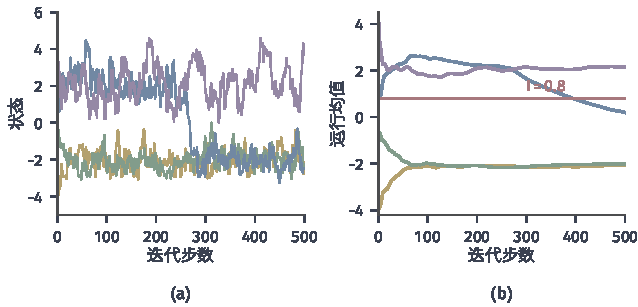
\includegraphics[width=108mm]{figures/07-probability/08-sampling-and-integration/matplotlib/budget-multistart/figure.pdf}
  \caption{双峰混合$0.3\,\mathcal{N}(-2,0.5^{2})+0.7\,\mathcal{N}(2,1)$上的随机游走Metropolis（步长$0.5$），四条链分别从$-4$（黄）、$-1$（绿）、$1$（蓝）、$4$（紫）启动，种子$0$到$3$。(a)~状态轨迹。(b)~$f(x)=x$的运行均值，红线为$I=0.8$。}
  \label{fig:budget-multistart}
\end{BookInlineFigure}

四条链之间的差异立刻暴露了问题，但把它们合起来平均并不能修正：合并均值约$-0.43$，因为四条链在两个峰上的时间比例反映的是初值的安排，而不是两个峰的概率$0.3$与$0.7$。所以多条链的分歧只能说明“当前的转移核在这个预算内不够用”，补救要回到转移核本身，例如加大步长（图~\ref{fig:budget-sampler-costs}中$s=4$的$\tau_{f}$约为$6.5$）。在预算分配上，这意味着要在单链延长带来的较小相关误差与多次启动带来的探索检查之间取舍：前者对已经走遍目标的链更经济，后者对可能多峰的目标是必要的保险。

\paragraph{成组采样的组内点数与重复数}
拉丁超立方与随机化准蒙特卡洛一次产生一组相关的点，第~\ref{chap:monte-carlo-integration-error}章说明误差要靠整组的独立重复来估计。设每组$n$个点，重复$R$组，总求值次数$N=nR$，另加点集准备的成本。两个参数的作用不同：$n$决定单组估计$Q$的精度，$R$是估计$\operatorname{Var}(Q)$时的独立观测数。

以随机移位网格$a_k=k/n$计算$\int_{0}^{1}\mathrm{e}^{u}\,\mathrm{d}u$为例。单组估计的方差有精确表达式，对大的$n$约为$(\mathrm{e}-1)^{2}/(12n^{2})$（第~\ref{chap:variance-reduction}章）。代入$n=N/R$，$R$组平均的方差为
\[
  \frac{\operatorname{Var}(Q_{n})}{R}\approx\frac{(\mathrm{e}-1)^{2}}{12n^{2}R}=\frac{(\mathrm{e}-1)^{2}R}{12N^{2}} .
\]
总点数固定时，组数越少，平均越准，因为单组方差随$n$下降得比$1/n$快。

可是只有$R$个组估计可用来估计方差，误差区间要用自由度$R-1$的$t$分位数$t_{R-1}$，形如$\bar{Q}\pm t_{R-1}s_{Q}/\sqrt{R}$。$R=2$时$t_{1}\approx12.7$，区间极宽。图~\ref{fig:budget-groups}(a)取$N=1024$，比较平均的均方根误差与区间的平均半宽：均方根误差随$R$单调增大，半宽在$R=4$到$8$附近最小（约$0.003$），$R=2$时约$0.0071$，$R=32$时约$0.0056$。图~\ref{fig:budget-groups}(b)是区间的实际覆盖率：$R=2$与$4$时约$0.93$，低于名义的$0.95$，因为单组估计$Q$的分布接近均匀而非正态；$R\ge8$后接近$0.95$。

\begin{BookInlineFigure}
  \centering
  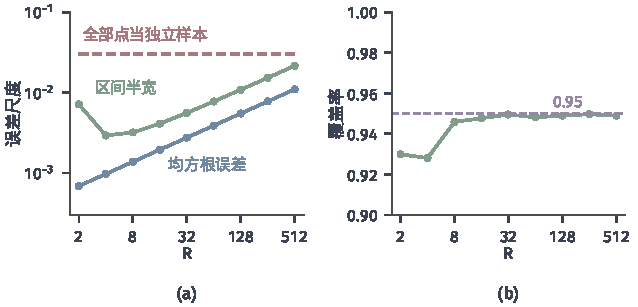
\includegraphics[width=108mm]{figures/07-probability/08-sampling-and-integration/matplotlib/budget-groups/figure.pdf}
  \caption{随机移位网格计算$\int_{0}^{1}\mathrm{e}^{u}\,\mathrm{d}u$，总点数$N=nR=1024$固定，横轴为组数$R$。(a)~蓝线为$R$组平均的均方根误差（精确公式），绿线为区间$\bar{Q}\pm t_{R-1}s_{Q}/\sqrt{R}$的平均半宽，红色虚线为把全部点当作独立样本时的半宽。(b)~该区间的覆盖率，紫色虚线为名义值$0.95$。(a)中的半宽与(b)均由$40000$次模拟得到（种子$3$）。}
  \label{fig:budget-groups}
\end{BookInlineFigure}

图中红色虚线是一个常见的错误：把全部$1024$个点的样本方差除以$1024$，得到半宽约$0.030$，比实际误差大一个数量级以上。这种做法在这里偏于保守，但它说明组内点不是独立样本，其样本方差与组平均的波动无关。对其他点集或被积函数，同样的错误也可能低估误差。综合两张图，总点数一定时，取十几到几十组通常是精度与误差估计可靠性之间的折中；若需要较准确的渐近区间，$R$还应更大，代价是单组的点数减少。

\section{方法选择}
\label{sec:budget-selection}

前三节给出了比较的尺子：误差口径、成本账和预算分配。还缺的是候选名单。一个方法能不能用，取决于目标分布和被积函数给了哪些可以计算的东西：能否计算分布函数的逆，能否逐点计算密度、只到一个常数因子还是完整归一化，能否对样本位置求导，是否知道某些辅助函数的精确期望。表~\ref{tab:budget-information}把前几章的方法按所需信息排列。

\begin{BookInlineTable}
  \centering
  \caption{可计算的信息与相应的方法}
  \label{tab:budget-information}
  \begin{tabular}{@{}p{44mm}p{62mm}@{}}
    \toprule
    可以计算的量 & 可用的方法 \\
    \midrule
    分位数函数 & 逆变换采样 \\
    混合成分或逐坐标条件分布 & 分步生成 \\
    有限包络常数下的密度比 & 拒绝采样 \\
    未归一化密度的比值 & MCMC，自归一化重要性采样 \\
    可采样且可计算密度的建议分布 & 重要性采样 \\
    期望已知的辅助函数 & 控制变量 \\
    精确的条件期望 & 条件期望降方差 \\
    层概率与层内条件抽样 & 分层采样 \\
    均匀输入下的生成映射 & 拉丁超立方，随机化准蒙特卡洛，对偶变量 \\
    被积函数对样本位置的导数 & 重参数化梯度 \\
    密度对参数的对数导数 & 得分函数梯度 \\
    \bottomrule
  \end{tabular}
\end{BookInlineTable}

名单只说明“可以用”，不说明“值得用”。一个方法可用而且理论上正确，并不意味着它在当前预算下比更朴素的方法有效。选择的依据始终是同一任务、同一误差口径下的总成本：先列出所有可用方案，再按第~\ref{sec:budget-costs}节的账估算每个方案的$\sigma^{2}c$和一次性开销，最后按预算决定。下面三小节分别对采样、方差控制和梯度估计做这件事。

\subsection{采样方法的选择}
\label{sec:budget-sampler-choice}

生成样本的方法大致按“需要的信息越多，结果越好”排列。直接生成（逆变换、分步生成）给出独立且精确服从目标的样本，每个样本成本固定；拒绝采样同样给出独立精确的样本，但每个输出平均要付出$M$个候选的成本；MCMC只需要未归一化密度的比值，代价是样本相关，而且要另行核验初值影响与探索范围。图~\ref{fig:budget-sampler-choice}把检查的顺序画成流程：从最强的信息问起，能用的第一个方法往往是成本最低的，但每个方法框右侧列出的量仍要逐项核对。

\begin{BookInlineFigure}
  \centering
  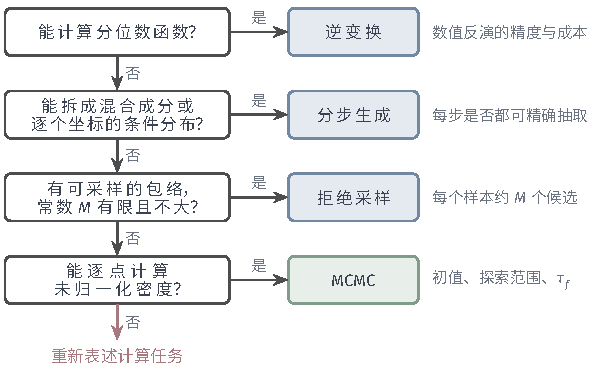
\includegraphics[width=101mm]{figures/07-probability/08-sampling-and-integration/tikz/budget-sampler-choice/figure.pdf}
  \caption{选择采样方法时依次检查的信息。左列从上到下要求的信息逐渐减少；每个方法框右侧是选定该方法后仍要比较的量：数值反演的精度、分步是否都能精确抽取、平均候选数$M$、链的初值影响与$\tau_{f}$。四项都不满足时（红色）需要改变计算任务的表述，例如换一个积分表示。}
  \label{fig:budget-sampler-choice}
\end{BookInlineFigure}

\paragraph{直接生成的数值精度}
分位数函数没有解析式时，逆变换要数值求解$F(x)=u$。用二分法在长度为$L$的区间上把$x$定位到容差$\eta$，需要约$\log_{2}(L/\eta)$次分布函数计算。容差带来一个确定性的偏差：输出不再精确服从$F$，而是服从相应的近似分布，第~\ref{chap:monte-carlo-integration-error}章说明这种偏差不随样本数减小。所以$\eta$要按最终的误差要求定：若$f$满足Lipschitz条件$\lvert f(x)-f(y)\rvert\le L_f\lvert x-y\rvert$，而数值反演把每个样本移动不超过$\eta$，则偏差不超过$L_f\eta$，取$L_f\eta$远小于$\varepsilon$即可，每个样本多付出的只是对数级的求值次数。

例如在长度$L=50$的区间上定位到$\eta=10^{-8}$，需要$\lceil\log_{2}(5\times10^{9})\rceil=33$次分布函数计算，比解析的逆变换贵几十倍，但仍可能比拒绝采样或MCMC便宜。分步生成要求每一步都能精确抽取；某一步只能近似时，整条生成链的偏差按同样方式核对。

\paragraph{拒绝采样的包络与尾部}
拒绝采样的成本由$M=\sup_{x}p(x)/q(x)$决定，而$M$有限要求包络在每个方向上的尾部不比目标轻。以$t_{3}$分布为目标，它的密度按$\lvert x\rvert^{-4}$衰减。用高斯包络$q_{1}=\mathcal{N}(0,2^{2})$时，比值
\[
  \frac{p(x)}{q_{1}(x)}\propto\Bigl(1+\frac{x^{2}}{3}\Bigr)^{-2}\mathrm{e}^{x^{2}/8}\to\infty,
\]
不存在有限的$M$；用Cauchy包络$q_{2}(x)=1/\bigl(\pi(1+x^{2})\bigr)$时比值有界，在$x=\pm1$处取最大值，网格计算得$M\approx1.30$。图~\ref{fig:budget-rejection-tails}画出这两种情形。

\begin{BookInlineFigure}
  \centering
  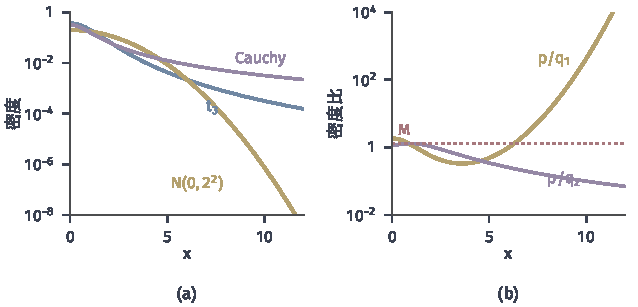
\includegraphics[width=108mm]{figures/07-probability/08-sampling-and-integration/matplotlib/budget-rejection-tails/figure.pdf}
  \caption{拒绝采样的包络必须覆盖目标的尾部。(a)~目标$t_{3}$（蓝）与两个包络的密度，对数纵轴：高斯$\mathcal{N}(0,2^{2})$（黄）在远处比目标轻得多，Cauchy（紫）比目标重。(b)~密度比$p/q$：对高斯包络无界，对Cauchy包络有界，红色点线为$M\approx1.30$。}
  \label{fig:budget-rejection-tails}
\end{BookInlineFigure}

若在高斯包络下强行取一个有限的“$M$”，例如只在$\lvert x\rvert\le6$上求最大值，算法仍然运行，但比值超过$M$的区域被系统地少接受，输出分布在尾部偏轻。这种错误不会使程序报错，样本的直方图在中心区域也与目标吻合；只有对依赖尾部的被积函数，例如$\mathbb{E}[X^{2}]$，偏差才显现出来。检查包络时，要对目标的支持和尾部给出解析的论证，而不是依赖样本。拒绝采样在高维的困难是另一回事：即使$M$有限，它也常随维数指数增长（第~\ref{chap:sample-generation}章），由式~\eqref{eq:budget-rejection-cost}，成本随之指数增长。

\paragraph{MCMC何时值得}
只有密度比可算时，MCMC往往是唯一的选择；但在直接生成或拒绝采样可用时，它通常不是最便宜的。图~\ref{fig:budget-sampler-costs}的双峰例子中，每个有效样本的成本是分步生成$4$、拒绝采样约$22$、最好的Metropolis约$52$。MCMC的优势在于每步只做局部的修改，在高维、各坐标强相关或只知道未归一化密度时，它的单步成本可以远低于任何直接生成方法。选择MCMC之后，比较的对象是转移核：步长、提议的形状、Gibbs与Metropolis--Hastings的组合等，比较的依据是针对所需被积函数的$c_{\mathrm{it}}\tau_{f}$，同时要有多次启动之类的检查（第~\ref{sec:budget-allocation}节）来确认链确实走遍了目标。

\subsection{方差控制方法的组合}
\label{sec:budget-vr-combination}

第~\ref{chap:variance-reduction}章的方法各自需要一种信息：重要性采样需要好的建议分布，控制变量需要期望已知且与$f$相关的辅助函数，条件期望降方差需要能精确计算的条件平均，分层需要层概率和层内条件抽样，对偶变量、拉丁超立方和随机化准蒙特卡洛需要从均匀输入出发的生成映射，共同随机数用于两个方案的差。它们可以叠加，例如先分层再在层内用对偶变量。叠加后的估计量是一个新的估计量，其期望、方差和成本都要重新计算，不能把各方法单独使用时的方差缩减倍数相乘或相加。

\paragraph{一个改进可能抵消另一个}
用$I=\mathbb{E}[\mathrm{e}^{U}]$、$U\sim\operatorname{Unif}(0,1)$比较几种组合，仍以每次计算$\mathrm{e}^{u}$为一个成本单位，辅助函数的计算视为免费。直接平均的单样本方差约为$0.2420$。对偶变量把$U$与$1-U$配成一对，每对的平均
\[
  g(U)=\frac{\mathrm{e}^{U}+\mathrm{e}^{1-U}}{2}
\]
要两次求值，按每次求值折算的方差约为$0.0078$。以$h(U)=U$作控制变量、取最优系数时，方差约为$0.0039$。

现在把两者叠加：先配对，再对配对后的估计用控制变量$U$。控制变量也要按同一种配对来算，即用$\bigl(U+(1-U)\bigr)/2$，而它恒等于$1/2$，没有任何波动可以利用。换一个角度，直接对$g(U)$与$U$求协方差：$g(u)=g(1-u)$关于$1/2$对称，而$U-1/2$反对称，于是
\[
  \operatorname{Cov}\bigl(g(U),U\bigr)=\mathbb{E}\bigl[g(U)(U-\tfrac12)\bigr]=\int_{0}^{1}g(u)\bigl(u-\tfrac12\bigr)\,\mathrm{d}u=0,
\]
因为把积分变量换成$1-u$后被积函数变号。对偶变量已经消去了$\mathrm{e}^{U}$中关于$1/2$的反对称部分，而$U$恰好只能解释这一部分。叠加的结果与单用对偶变量相同，比单用控制变量还差一倍。

反过来，若控制函数选在对偶变量留下的对称部分上，例如$h(U)=(U-\tfrac12)^{2}$，叠加后每次求值的方差降到约$2.2\times10^{-7}$。分层与对偶变量的叠加也类似：$4$层比例分层的方差约为$0.0165$，在每层内再配对后降到约$3.4\times10^{-5}$。图~\ref{fig:budget-vr-combos}把这些数并列，对数横轴上相差几个数量级。

\begin{BookInlineFigure}
  \centering
  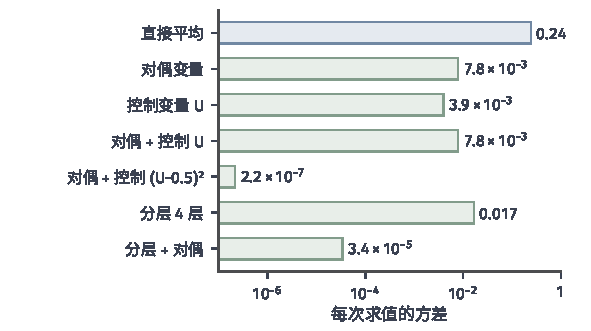
\includegraphics[width=100mm]{figures/07-probability/08-sampling-and-integration/matplotlib/budget-vr-combos/figure.pdf}
  \caption{计算$\mathbb{E}[\mathrm{e}^{U}]$时几种方差控制及其组合按每次求值折算的方差（数值积分精确计算，控制函数视为免费，控制系数取最优值）。蓝色为直接平均。“对偶 + 控制$U$”与单用对偶变量相同，因为配对后的控制量恒为$1/2$；控制函数改为对称的$(U-0.5)^{2}$后方差骤降。}
  \label{fig:budget-vr-combos}
\end{BookInlineFigure}

这组数字的教训是一般的：每种方法消去被积函数的某一部分波动，组合的效果取决于这些部分是否重叠。重叠时后一种方法无事可做，还白白付出成本；互补时效果可以远超任一方法单用。所以组合之后要按实际的估计量重新计算，第~\ref{chap:variance-reduction}章对单个方法证明的方差公式不能拼接使用。

\paragraph{高维均匀输入与变换后的函数}
拉丁超立方和随机化准蒙特卡洛作用在$[0,1)^{d}$的均匀输入上，被平均的是$F=f\circ T$，$T$是第~\ref{chap:sample-generation}章的生成映射。它们的改进依赖$F$的性质，而不是$f$的性质。拉丁超立方逐坐标均匀覆盖，对接近各坐标函数之和的$F$效果好，对主要由坐标间相互作用决定的$F$几乎无改进，有限样本下甚至可能不如独立抽样。随机化准蒙特卡洛的快速收敛要求$F$有一定的光滑性；若$T$是高斯的逆分布函数$\Phi^{-1}$，即使$f$光滑，$F$在立方体边界附近也无界，若$f$含示性函数，$F$在立方体内部有间断，两者都会使误差衰减变慢。选择这类方法时，要先检查变换后的函数，再按第~\ref{sec:budget-allocation}节选定$n$与$R$，误差只用组间方差估计。

\paragraph{两个方案的差}
比较两个方案的期望差$\mathbb{E}[A]-\mathbb{E}[B]$时，共同随机数用同一输入$U$生成$A(U)$与$B(U)$，由
\[
  \operatorname{Var}\bigl(A(U)-B(U)\bigr)=\operatorname{Var}(A)+\operatorname{Var}(B)-2\operatorname{Cov}\bigl(A(U),B(U)\bigr),
\]
正协方差越大，差的方差越小。与其他方法组合时要检查这种正协方差是否保留。若两个方案各自使用不同的重要性采样建议分布，同一个$U$在两边对应不同的样本位置，耦合可能失效；若两边都用逆变换且输出对输入单调同向，耦合通常最强。

用第~\ref{chap:variance-reduction}章的例子算一下：$A=\min\{X,1\}$，$X\sim\operatorname{Exp}(1)$；$B=\min\{Y,1\}$，$Y\sim\operatorname{Exp}(1.25)$；期望差约为$0.0613$。数值积分给出$\operatorname{Var}(A)\approx0.1289$、$\operatorname{Var}(B)\approx0.1291$。按差值的单对方差计，三种耦合方式的结果是
\[
  \underbrace{0.258}_{\text{独立输入}},\qquad\underbrace{0.0038}_{X,Y\text{用同一个}U},\qquad\underbrace{0.506}_{X\text{用}U,\ Y\text{用}1-U} .
\]
同向耦合把方差缩小约$68$倍；若误把对偶变量的反向配对用在差值上，协方差变负，方差反而比独立输入大近一倍。可见同一个“共用随机数”的操作，效果完全取决于两边输出对输入的单调方向。组合前后应各用一次小规模试运行，直接估计$\operatorname{Cov}(A,B)$，而不是假定它为正。

\subsection{梯度估计的选择}
\label{sec:budget-gradient-choice}

第~\ref{chap:expectation-gradient-estimation}章的三种表示分别依赖不同的条件。分布不随参数变化时，直接对被积函数求导；样本可写成$X=T_{\bm{\theta}}(\varepsilon)$且被积函数对样本位置可微时，用重参数化；能计算$\nabla_{\bm{\theta}}\ln p_{\bm{\theta}}$时，用得分函数，它不要求$f$对样本位置可微。离散样本空间上没有沿样本路径的导数，重参数化不能直接使用；状态数很少时还有一个更好的选择：直接求和。例如$X\sim\operatorname{Bern}(\theta)$时，$J(\theta)=\theta f(1)+(1-\theta)f(0)$，梯度$f(1)-f(0)$用两次求值就精确算出，没有任何随机误差。

条件都满足时，比较的依据仍是同一梯度任务下的偏差、方差与成本。不能预设重参数化总是方差更小，也不能预设得分函数总是更通用就更好。下面两个例子分别给出相反的结论。

\paragraph{被积函数振荡时}
设$X=\theta+\varepsilon$，$\varepsilon\sim\mathcal{N}(0,1)$，$f(x)=\sin(kx)$。由标准高斯的特征函数$\mathrm{e}^{-b^{2}/2}$，
\[
  J(\theta)=\sin(k\theta)\,\mathrm{e}^{-k^{2}/2},\qquad J'(\theta)=k\cos(k\theta)\,\mathrm{e}^{-k^{2}/2}.
\]
密度$\varphi(x-\theta)$的得分为$x-\theta$，在样本处等于$\varepsilon$，两种单样本估计分别是
\[
  \hat{g}_{\mathrm{R}}=k\cos\bigl(k(\theta+\varepsilon)\bigr),\qquad\hat{g}_{\mathrm{S}}=\sin\bigl(k(\theta+\varepsilon)\bigr)\,\varepsilon .
\]

用$\cos^{2}y=(1+\cos2y)/2$、$\sin^{2}y=(1-\cos2y)/2$及
\[
  \mathbb{E}\bigl[\cos(a+b\varepsilon)\bigr]=\cos a\,\mathrm{e}^{-b^{2}/2},\qquad\mathbb{E}\bigl[\varepsilon^{2}\cos(a+b\varepsilon)\bigr]=\cos a\,(1-b^{2})\,\mathrm{e}^{-b^{2}/2},
\]
两者的二阶矩分别为
\[
  \frac{k^{2}}{2}\bigl(1+\cos(2k\theta)\,\mathrm{e}^{-2k^{2}}\bigr),\qquad\frac12-\frac12\cos(2k\theta)\,(1-4k^{2})\,\mathrm{e}^{-2k^{2}} .
\]
减去梯度的平方即得方差。$k$较大时重参数化的方差约为$k^{2}/2$，得分函数的方差约为$1/2$：重参数化把$f$的导数带进估计，振荡越快，导数的幅度越大；得分函数只用到$f$的值，而$\lvert\sin\rvert\le1$。

图~\ref{fig:budget-gradient-variance}(a)取$\theta=0.3$，两条曲线在$k\approx1.09$相交。$k=0.5$时重参数化的方差约$0.0071$，得分函数约$0.31$，前者好四十多倍；$k=3$时前者约$4.50$，后者约$0.50$，后者好九倍。重参数化还要计算$f'$，每个样本的成本通常更高，所以$k$较大时得分函数在工作量归一化方差上的优势更明显。$2\times10^{6}$个样本的模拟（种子$1$）在$k=1$与$k=3$处与上面的公式相差不到$1\%$。

\begin{BookInlineFigure}
  \centering
  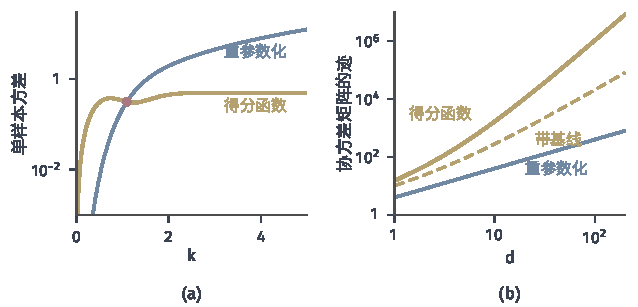
\includegraphics[width=108mm]{figures/07-probability/08-sampling-and-integration/matplotlib/budget-gradient-variance/figure.pdf}
  \caption{同一梯度任务下两种估计的单样本方差。(a)~$J(\theta)=\mathbb{E}[\sin(kX)]$，$X\sim\mathcal{N}(\theta,1)$，$\theta=0.3$：蓝线为重参数化，黄线为得分函数，红点为交点$k\approx1.09$。(b)~$J(\bm{\theta})=\mathbb{E}\lVert\bm{X}\rVert_2^{2}$，$\bm{X}\sim\mathcal{N}(\bm{\theta},\bm{I}_d)$，$\bm{\theta}=\bm{0}$：协方差矩阵的迹随维数$d$的变化，黄色虚线为得分函数减去基线$d$之后。}
  \label{fig:budget-gradient-variance}
\end{BookInlineFigure}

\paragraph{维数增大时}
设$\bm{X}=\bm{\theta}+\bm{\varepsilon}$，$\bm{\varepsilon}\sim\mathcal{N}(\bm{0},\bm{I}_d)$，$f(\bm{x})=\lVert\bm{x}\rVert_2^{2}$，在$\bm{\theta}=\bm{0}$处求梯度，真值为$\bm{0}$。

重参数化的估计是$2\bm{X}$，协方差矩阵为$4\bm{I}_d$，迹为$4d$。得分函数的估计是$\lVert\bm{X}\rVert_2^{2}\bm{X}$，由于真值为零，迹等于二阶矩$\mathbb{E}\lVert\bm{\varepsilon}\rVert_2^{6}$。$S=\lVert\bm{\varepsilon}\rVert_2^{2}$服从$\chi^{2}_{d}$，其各阶矩为
\[
  \mathbb{E}[S]=d,\qquad\mathbb{E}[S^{2}]=d(d+2),\qquad\mathbb{E}[S^{3}]=d(d+2)(d+4),
\]
于是
\[
  \operatorname{tr}\bm{\Sigma}_{\text{得分}}=\mathbb{E}\lVert\bm{\varepsilon}\rVert_2^{6}=d(d+2)(d+4).
\]
减去与样本独立的基线$b=\mathbb{E}\lVert\bm{X}\rVert_2^{2}=d$后，估计变为$(\lVert\bm{X}\rVert_2^{2}-d)\bm{X}$，其迹为
\[
  \begin{aligned}
    \mathbb{E}\bigl[(S-d)^{2}S\bigr]&=\mathbb{E}[S^{3}]-2d\,\mathbb{E}[S^{2}]+d^{2}\,\mathbb{E}[S]\\
    &=d(d+2)(d+4)-2d^{2}(d+2)+d^{3}=2d^{2}+8d .
  \end{aligned}
\]
基线把三次增长降成二次，但仍比重参数化的$4d$大约$d/2$倍。图~\ref{fig:budget-gradient-variance}(b)在对数坐标上显示了这三条曲线：$d=100$时分别为$400$、约$1.06\times10^{6}$与$20\,800$。这里重参数化每个样本要计算一次$\nabla f$，用反向自动求导时其成本是$f$的常数倍，与$d$无关，抵消不了$d/2$倍的方差差距。

\paragraph{可微性的条件}
重参数化的前提是把求导与求期望交换。$f$不连续时这一步可能失败而不报错。取$f(x)=\mathbf{1}_{\{x>0\}}$，$X=\theta+\varepsilon$，则$J(\theta)=\Phi(\theta)$，梯度为$\varphi(\theta)>0$；但对几乎每个$\varepsilon$，$\mathbf{1}_{\{\theta+\varepsilon>0\}}$在$\theta$附近是常数，路径导数为零，重参数化的估计恒为$0$。得分函数的估计$\mathbf{1}_{\{X>0\}}(X-\theta)$在这里无偏。所以选择重参数化之前，要先按第~\ref{chap:expectation-gradient-estimation}章检查交换条件，而不是看程序能否算出导数。

综合起来，梯度估计的选择依次回答四个问题：分布是否随参数变化；样本空间是否离散且小到可以直接求和；能否沿生成映射求导，且交换条件成立；能否计算得分。满足条件的估计都列出后，按式~\eqref{eq:budget-vector-mse}的迹或所需方向上的方差，乘以每个样本的成本来比较。参数怎样依据这些梯度更新，可参考\BookChapterRef{chap:stochastic-gradient-methods}{卷五第13章“随机梯度方法”}，那里梯度估计的方差直接影响步长的选择与收敛速度。

\section{试运行与停止}
\label{sec:budget-stopping}

前面的分配与选择都用到了事先不知道的量：单样本方差、成本、包络常数、$\tau_{f}$、建议分布的参数。它们只能由试运行估计。试运行的结果一旦用来做决定，后面的计算就依赖于这些随机的决定，原先对固定方法证明的结论是否还成立，需要重新检查。同样的问题出现在“何时停止”上：按事先固定的样本数停止，与看着结果决定何时停止，是两种不同的随机程序。

\paragraph{试运行与正式计算分开}
试运行的作用是估计成本、波动以及方法的参数，例如图~\ref{fig:budget-pilot-size}中的$\hat{\lambda}$、式~\eqref{eq:budget-neyman-cost}中的$\sigma_k$、图~\ref{fig:budget-sampler-costs}中的步长。正式计算用新的独立随机数。这样，给定试运行结果时，正式计算就是一个参数固定的普通方法，第~\ref{chap:monte-carlo-integration-error}章和第~\ref{chap:variance-reduction}章对固定方法证明的无偏性、方差公式和渐近区间都可以在条件意义下直接使用。

试运行的样本可不可以并入最终的平均？若试运行只是从固定的分布抽样且不参与任何选择，并入没有问题。若试运行被用来在几个方法中挑选，问题就来了：设对两个同样无偏的方法各做一次试运行，选估计方差较小的一个，再报告它在试运行中的估计。被选中的往往是试运行时“碰巧波动较小”的那一个，而对偏斜的被积函数，波动偏小常常伴随着均值偏小（漏掉了大的贡献），于是报告的数系统地偏低。最稳妥的做法是只把试运行用于决定，最终估计只用正式计算的样本；试运行所占的预算按式~\eqref{eq:budget-pilot-opt}本来就只是一小部分。

\paragraph{固定转移核与持续调参}
MCMC的步长、提议协方差等参数通常靠试运行调整。调整的依据应当是第~\ref{sec:budget-costs}节的$c_{\mathrm{it}}\tau_{f}$，而不只是接受率：图~\ref{fig:budget-sampler-costs}中接受率最高的$s=1$恰恰最贵。试运行结束后把参数固定，正式计算的链就是一条时间齐次的Markov链，转移核保持目标不变；但链是否从初值的影响中走出来、是否走遍目标、相关误差多大，仍要按第~\ref{chap:monte-carlo-integration-error}章逐项核对，参数选得好并不能免除这些检查。

一个诱人的做法是不停止调参：在正式计算中继续根据已走过的轨迹修改转移核。每个可能用到的核都以$\pi$为不变分布，看起来整体也应当正确。下面的例子说明这个推理不成立。状态空间为$\{1,2\}$，目标$\pi=(\tfrac12,\tfrac12)$。核$K_{A}$是恒等转移（停在原处），核$K_{B}$以概率$\tfrac12$去往每个状态，二者都保持$\pi$不变：
\[
  \pi K_{A}=\pi,\qquad\pi K_{B}=\bigl(\tfrac12,\tfrac12\bigr)=\pi .
\]
调整规则是：当前在状态$1$时用$K_{A}$，在状态$2$时用$K_{B}$。图~\ref{fig:budget-adaptive-trap}画出两个核及其组合。

\begin{BookInlineFigure}
  \centering
  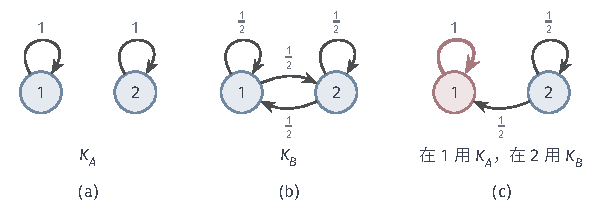
\includegraphics[width=101mm]{figures/07-probability/08-sampling-and-integration/tikz/budget-adaptive-trap/figure.pdf}
  \caption{每个核都保持目标不变，按轨迹选核却可能破坏它。状态空间$\{1,2\}$，目标$\pi=(\tfrac12,\tfrac12)$。(a)~$K_{A}$为恒等转移。(b)~$K_{B}$的每个转移概率都是$\tfrac12$。(c)~在状态$1$用$K_{A}$、在状态$2$用$K_{B}$的组合：状态$1$（红）成为吸收态。}
  \label{fig:budget-adaptive-trap}
\end{BookInlineFigure}

组合后的过程从状态$1$出发永远停在$1$，从状态$2$出发每步以$\tfrac12$的概率跳到$1$并从此停住。从$\pi$启动，$\mathbb{P}(X^{(0)}=2)=\tfrac12$，此后每步留在$2$的概率为$\tfrac12$，所以
\[
  \mathbb{P}\bigl(X^{(t)}=2\bigr)=\frac12\Bigl(\frac12\Bigr)^{t},\qquad\mathbb{P}\bigl(X^{(t)}=1\bigr)=1-2^{-(t+1)}\to1 .
\]
过程收敛到点质量$\delta_{1}$，而不是$\pi$。问题在于“用哪个核”依赖当前状态，组合起来的是另一个转移核，它不再保持$\pi$不变。不变性是对固定的核说的，不能由“每次所用的核都保持$\pi$”推出整体保持$\pi$。

持续调参并非不可行，但需要额外的理论。大致说，要求调整的幅度随时间趋于零，并且所用的核对目标的收敛速度有一致的控制，才能证明过程的边缘分布趋于$\pi$、平均满足大数律。这些条件涉及一般Markov链的遍历理论，证明较长，相关的收敛工具可参考\BookChapterRef{chap:discrete-time-stochastic-processes}{卷九第3章“离散时间随机过程”}。本卷采用更简单的做法：试运行中调参，正式计算中固定。

\paragraph{经验稳定的局限}
试运行和停止判断都要看结果是否“稳定”，但有限记录上的稳定不能证明正确。下面三种现象都会让运行均值在错误的值附近显得平稳。

第一种是稀有的大贡献。若对积分起主要作用的区域概率很小，有限的试运行可能一个样本也没有落进去，估计的方差为零，一切看起来都很精确。图~\ref{fig:budget-pilot-size}的例子之所以平稳，是因为$q_{0}=\operatorname{Exp}(1/2)$落入尾部的概率是$\mathrm{e}^{-2}\approx0.135$；若试运行直接从$\operatorname{Exp}(1)$抽样，这个概率只有$0.018$，$n_{0}=20$时有约$69\%$的试运行完全看不到尾部。

第二种是权重集中。仍算$I=\mathbb{P}(X>4)$，但用尾部比目标还轻的建议分布$q=\operatorname{Exp}(2.2)$。权重$w(y)=\mathrm{e}^{-y}/(2.2\,\mathrm{e}^{-2.2y})$在尾部指数增长，加权变量在$q$下的二阶矩为
\[
  \int_{4}^{\infty}\frac{\mathrm{e}^{-2y}}{2.2\,\mathrm{e}^{-2.2y}}\,\mathrm{d}y=\frac{1}{2.2}\int_{4}^{\infty}\mathrm{e}^{0.2y}\,\mathrm{d}y=\infty,
\]
估计无偏而方差无穷。图~\ref{fig:budget-weight-instability}画出三次独立运行：每次在前几千个样本内都没有命中尾部，估计为零；命中后估计跳起，之后每隔一段又被一个更大的权重抬升。$10^{6}$个样本后三次的估计约为$0.0149$、$0.0164$、$0.0163$，都低于$I\approx0.0183$。右图是最大的一项在累计和中的占比：它长时间接近$1$，说明整个估计由一两个样本决定。

\begin{BookInlineFigure}
  \centering
  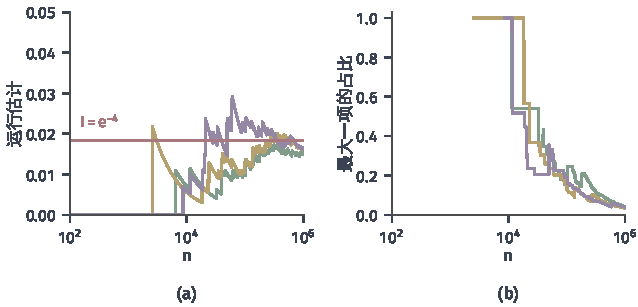
\includegraphics[width=108mm]{figures/07-probability/08-sampling-and-integration/matplotlib/budget-weight-instability/figure.pdf}
  \caption{建议分布尾部过轻时的重要性采样：目标$I=\mathbb{P}(X>4)$，$X\sim\operatorname{Exp}(1)$，从$\operatorname{Exp}(2.2)$抽样，加权变量方差无穷。三种颜色是三次独立运行（种子$11$、$12$、$13$）。(a)~运行估计，红线为真值。(b)~累计和中最大一项所占的比例。}
  \label{fig:budget-weight-instability}
\end{BookInlineFigure}

第三种是链之间的分歧。图~\ref{fig:budget-multistart}中每条链的运行均值都在某个值附近平稳下来，只有并排比较多条从不同初值出发的链，才看得出它们停在不同的地方。

这三种现象对应三种检查：对被积函数与建议分布的尾部做解析的矩估计，监视最大权重的占比，比较多条独立启动的链。它们能发现问题，但都不能证明没有问题：若所有链都错过了同一个峰，或所有试运行都没有触及同一个稀有区域，检查也全部通过。经验检查只能补充理论条件，不能代替它。

\paragraph{固定样本数与数据依赖的停止}
最常见的停止方式是看着误差估计做决定：每增加一些样本就计算一次$z\,s_n/\sqrt{n}$，一旦它小于容差$\varepsilon$就停止，报告$\bar{X}_n\pm z\,s_n/\sqrt{n}$。称这类规则为\term{序贯停止规则}（sequential stopping rule），停止时的样本数$N_{\varepsilon}$是随机的，依赖于样本本身。固定样本数的中心极限定理说的是$n$不随数据变化的情形，不能直接搬到$N_{\varepsilon}$上。

机制在偏斜分布上最清楚。设$f(U)=U^{-1/3}$，即$X$服从$[1,\infty)$上指数为$3$的Pareto分布，$I=1.5$，$\sigma^{2}=0.75$，右尾较重。一段样本恰好没有出现大值时，$s_n$偏小，均值也偏小；停止规则偏偏在这种时候触发，于是停下来时的估计系统地偏低，区间又偏窄。取$z=1.96$、最少$10$个样本、每增加一个样本检查一次，$20000$次模拟（种子$5$）的结果如图~\ref{fig:budget-sequential-coverage}。$\varepsilon=0.1$时，用真实$\sigma^{2}$定出的固定样本数$n=\lceil1.96^{2}\times0.75/0.01\rceil=289$，区间覆盖率约$0.925$；序贯规则平均只用了约$174$个样本就停止，覆盖率只有约$0.77$。

\begin{BookInlineFigure}
  \centering
  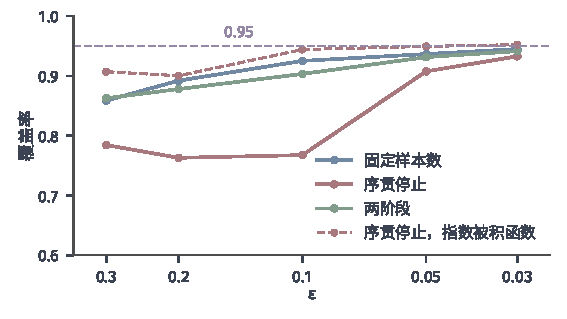
\includegraphics[width=96mm]{figures/07-probability/08-sampling-and-integration/matplotlib/budget-sequential-coverage/figure.pdf}
  \caption{名义$95\%$区间在三种停止方式下的实际覆盖率，横轴为目标半宽$\varepsilon$（向右减小）。实线为偏斜的被积函数$U^{-1/3}$（$I=1.5$，$\sigma^{2}=0.75$）：蓝线用真实方差定出固定样本数，红线在半宽首次小于$\varepsilon$时停止（最少$10$个样本），绿线先用$30$个独立试运行样本估计方差再定样本数。红色虚线为序贯停止用于$\mathrm{e}^{U}$的情形。每点$20000$次模拟（种子$5$）。}
  \label{fig:budget-sequential-coverage}
\end{BookInlineFigure}

$\varepsilon$变小时三条实线都向$0.95$靠拢：$\varepsilon=0.03$时固定样本数、两阶段与序贯规则的覆盖率分别约为$0.945$、$0.941$、$0.933$。对较对称的$\mathrm{e}^{U}$，序贯规则在$\varepsilon=0.1$时已有约$0.944$。这与一个渐近结论相符：若$0<\sigma^{2}<\infty$，并且停止规则要求的最少样本数随$\varepsilon\to0$趋于无穷（或在判据中加入防止过早停止的修正项），则$\varepsilon\to0$时覆盖率趋于名义值。它的证明需要随机样本数下的中心极限定理，篇幅较长，这里只说明其含义：数据依赖的停止只在误差要求足够严、停止时样本足够多时才近似可靠，对给定的有限$\varepsilon$没有保证。

既想依据数据定样本数、又要保留固定样本数的保证，可以把决定和估计分开，称为\term{两阶段方法}（two-stage procedure）：先用独立的试运行估计方差，据此定出正式样本数，再用新样本计算。

\begin{lemma}
\label{lem:budget-two-stage}
设试运行样本$\bm{Y}$与正式样本$X_1,X_2,\dots$相互独立，$X_i$独立同分布，$\mathbb{E}[X_i]=I$，$\operatorname{Var}(X_i)=\sigma^{2}<\infty$。正式样本数$N$是$\bm{Y}$的函数，取正整数值。令$\hat{I}=N^{-1}\sum_{i=1}^{N}X_i$，则
\begin{equation}
  \mathbb{E}\bigl[\hat{I}\mid\bm{Y}\bigr]=I,\qquad\operatorname{Var}\bigl(\hat{I}\mid\bm{Y}\bigr)=\frac{\sigma^{2}}{N},\qquad\operatorname{Var}(\hat{I})=\sigma^{2}\,\mathbb{E}\Bigl[\frac1N\Bigr].
  \label{eq:budget-two-stage}
\end{equation}
\end{lemma}

\begin{proof}
给定$\bm{Y}=\bm{y}$时$N=n(\bm{y})$是确定的正整数。由独立性，在这一条件下$X_1,X_2,\dots$的联合分布不变，仍独立同分布、均值$I$、方差$\sigma^{2}$。于是$n(\bm{y})$个样本的平均的条件期望为$I$，条件方差为$\sigma^{2}/n(\bm{y})$，这就是前两个等式。

由全期望公式，
\[
  \mathbb{E}[\hat{I}]=\mathbb{E}\bigl[\mathbb{E}[\hat{I}\mid\bm{Y}]\bigr]=I .
\]
由全方差公式，
\[
  \operatorname{Var}(\hat{I})=\mathbb{E}\bigl[\operatorname{Var}(\hat{I}\mid\bm{Y})\bigr]+\operatorname{Var}\bigl(\mathbb{E}[\hat{I}\mid\bm{Y}]\bigr)=\mathbb{E}\Bigl[\frac{\sigma^{2}}{N}\Bigr]+\operatorname{Var}(I)=\sigma^{2}\,\mathbb{E}\Bigl[\frac1N\Bigr],
\]
因为常数$I$的方差为零。
\end{proof}

引理的要点是$N$只依赖试运行。条件在试运行上，正式计算就是固定样本数的计算，固定样本数的渐近区间在条件意义下适用；$N$越大，条件覆盖率越接近名义值。图~\ref{fig:budget-sequential-coverage}的绿线用$30$个试运行样本的标准差$s_{0}$定出
\[
  N=\max\bigl\{30,\ \lceil z^{2}s_{0}^{2}/\varepsilon^{2}\rceil\bigr\},
\]
其覆盖率略低于用真实方差的蓝线（$\varepsilon=0.1$时约$0.903$对$0.925$），而明显高于序贯规则。差距来自试运行：$s_{0}$偏小时$N$偏小，最终区间可能比$\varepsilon$宽，也就是精度没有达标；但估计本身在条件意义下仍然无偏，不再出现序贯规则那种系统偏低。若$\bm{Y}$与正式样本不独立，例如把试运行样本并入最终平均，引理的条件就不满足。

用积分$\mathrm{e}-1$走一遍两阶段方法，取$\varepsilon=0.01$、$z=1.96$，随机数种子固定为$2026$。$30$个试运行样本的标准差为$s_{0}\approx0.426$，比真实的$\sigma\approx0.492$偏小，于是
\[
  N=\Bigl\lceil\frac{1.96^{2}\times0.426^{2}}{10^{-4}}\Bigr\rceil=6984,
\]
少于用真实方差算出的约$9300$。用新的$6984$个样本得到均值约$1.7290$，标准差约$0.493$，区间半宽为
\[
  1.96\times\frac{0.493}{\sqrt{6984}}\approx0.0116 .
\]
半宽超过了要求的$0.01$，这是试运行低估方差的后果；但这个区间如实反映了正式样本的波动，其下端约为$1.7174$，覆盖了$\mathrm{e}-1\approx1.7183$。若精度必须达标，可以把这次结果当作新的试运行，再定一次样本数，并仍用新样本计算。

最后，“预算用完就停”是固定预算的停止，样本数不依赖于样本的取值，固定样本数的结论适用。若每个样本的成本本身随机（例如拒绝采样的候选数），按预算停止时的样本数也随机，但它只依赖成本，不依赖被积函数的取值；拒绝采样中接受与否与被接受样本的取值独立，这种停止不会造成上面那种偏差。

\section{本章小结}
\label{sec:budget-summary}

本章把采样生成、误差分析、方差控制与梯度表示放到同一本账上，回答“给定任务和预算，怎样安排一次随机计算”。回到章首的问题：计算$I=\mathbb{P}(X>4)$，要求$95\%$把握下相对误差不超过$10\%$。$I\approx0.0183$离零较远，相对要求有意义，按式~\eqref{eq:budget-mixed-tolerance}给一个绝对下限以防目标接近零即可。直接平均约需$20\,600$个样本；先用几十个试运行样本拟合$\operatorname{Exp}(\lambda)$建议分布，再做重要性采样，约需$1990$个正式样本，成本约$3000$。两者都在$10^{5}$的预算之内，后者约省$85\%$；正式样本数按两阶段方法由试运行确定，最终估计只用正式样本。

\paragraph{误差与成本的口径}
误差要求先要说清是均方误差、指定概率下的绝对误差，还是相对误差；目标可能为零时用混合容差。无偏方法之间比较工作量归一化方差$\sigma^{2}c$，它在固定预算与固定精度两种提法下给出同一排序；有偏方法还要选择控制偏差的参数，近似链的例子中最优安排使均方根误差只按$B^{-1/3}$下降。成本要计入被拒绝的候选、矩阵分解与试运行等一次性开销，以及链的初始化；相关链按有效样本计成本，而有效样本数依赖被积函数，抽稀只节省存储。

\paragraph{预算的分配}
试运行的最优规模按$\sqrt{C}$增长，占预算的比例随预算增大而缩小，最终误差对它的具体取值通常不敏感。分层的最优分配在考虑成本时为$n_k\propto p_k\sigma_k/\sqrt{c_k}$。对单峰且混合良好的链，一条长链的均方误差最小，多条短链各自带着初值偏差；多次启动的价值在于暴露链没有走遍目标。成组随机化中，组内点数$n$决定精度，组数$R$决定误差估计的可靠性，不能把全部点当作独立样本估计误差。

\paragraph{方法的选择}
可用的方法由可计算的信息决定：分位数、条件分布、有限包络、密度比、期望已知的辅助函数、可微的生成映射或得分。在可用的方法之间，以同一任务的总成本比较：一维双峰例子中直接生成比最好的Metropolis便宜十几倍；方差控制的组合要重新计算，对偶变量之后再用控制变量$U$毫无收益，而换成对称的控制函数则收益巨大；梯度估计没有普遍的优劣，被积函数振荡时得分函数方差小，维数高时重参数化方差小，被积函数不连续时重参数化可能静默地给出错误结果。

\paragraph{试运行与停止的条件}
试运行只用于决定，正式计算用新的随机数，固定方法的结论才在条件意义下适用。MCMC在试运行中调参、正式计算中固定转移核；按轨迹持续换核，即使每个核都保持目标不变，整体也可能收敛到错误的分布。稀有贡献、权重集中与链间分歧都能让有限记录显得平稳，经验检查只能发现问题，不能证明正确。依据误差估计决定何时停止会使偏斜被积函数的区间系统性地失效，只在要求足够严时渐近可靠；把定样本数与计算估计分开的两阶段方法保留了固定样本数的结论。

最终报告一次随机计算，应分别给出计算偏差（及其来源，如近似生成或初值）、随机波动（及其估计方式和所依据的条件）以及实际成本。这里的“精度”是对一个确定的数做随机计算时的精度：分布已知、积分待算，随机性完全来自我们所用的随机数，可以通过增加计算来减小。它与由有限数据推断未知总体时的精度是两回事，后者的误差来自数据本身，加大计算量无法消除，相应的理论见\BookChapterRef{chap:parametric-statistical-inference}{卷八第1章“参数化统计推断”}。

